% !TEX root = ../../thesis.tex

\section{Power System State Estimation}\label{sec:application}
We first introduce the physical layer model of an interconnected power system comprising several synchronous generators and buses, and then introduce a graph-theoretic model to describe the communication network which interconnects the wide-area and local controllers of the power system. Figure~\ref{ps} illustrates the interactions between the physical and cyber layers in the system. Note that the components of the system and the notation used
in this figure will be introduced throughout this section. Finally, we introduce two categories of cyber attacks that can potentially corrupt measurements and degrade the system's performance.

\begin{figure*}[t]
\begin{center}
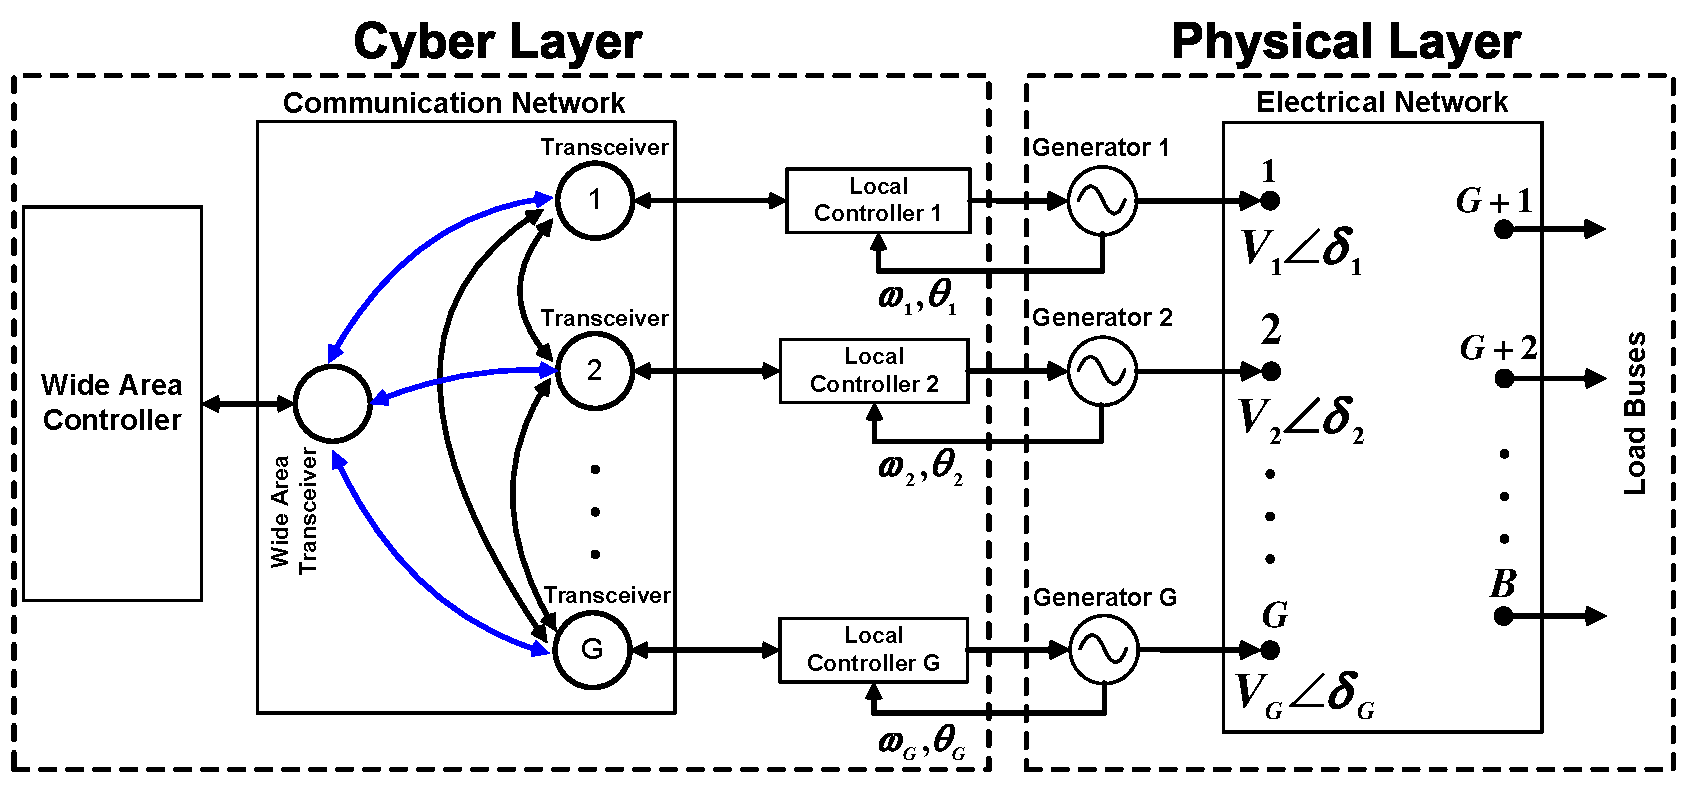
\includegraphics[width=\textwidth]{chapters/se_nonlinear/figures/ps}\caption{A graphical depiction of the power system including both the physical and cyber layers.}\label{ps}
\end{center}
\end{figure*}



\subsection{Physical Layer Model}
Consider a power system comprising $G$ generators and $B$ buses. We assume that $G$ of the buses are generator buses, and that the remaining buses ($B-G$ buses) are load buses. Let $\mathcal{B}$ and $\mathcal{V}$ denote the set of buses and transmission lines, respectively. Here, we assume that the corresponding graph $\mathcal{H}(\mathcal{B},\mathcal{V})$ is connected, and that the network topology is fixed and known.

\textbf{Load buses:} Let $V_i$ and $\delta_i$ denote the magnitude and phase angle of the voltage phasor, respectively, at load bus $i\in\mathcal{L}$ where $\mathcal{L}$ is the set of load buses ($|\mathcal{L}|=B-G$). Let $P_i^e$ be the total active power leaving bus $i$ (i.e., the real power drawn by the load
at bus $i$ equals $-P_i^e$). $P_i^e$ can be computed by
\begin{align}
\label{load_bus}&P_i^e=\sum_{j\in\mathcal{B}}{{V_i V_j |y_{ij}|~\text{sin}(\delta_i-\delta_j+\phi_{ij})}}
\end{align}
where $y_{ij}=g_{ij}+\sqrt{-1} b_{ij}$ is the admittance of the line between buses $i$ and $j$, and $\phi_{ij}$ equals $\text{arctan}(g_{ij}/b_{ij})$. Note that $g_{ij}=g_{ji}\ge0$ and $b_{ij}=b_{ji}>0$ are the conductance and susceptance of the line between buses $i$ and $j$, respectively.




\textbf{Generator buses:} Let $\widehat{E_i}=E_i \phase{\theta_i}$ denote the internal voltage phasor of the generator connected to bus $i\in\mathcal{G}$ where $\mathcal{G}$ is the set of generator buses in the system. According to the synchronous machine theory, $E_i$ is constant and $\theta_i$ is the angular position of the generator rotor as measured with respect to a synchronous reference rotating at the nominal system electrical frequency $\omega_0$. We assume that the voltages at the generator buses are controlled via droop control, and that all the generator terminal buses are equipped with fast response energy storage units which are controlled via local and wide area controllers. Under these assumptions, for a synchronous generator connected to bus $i\in\mathcal{G}$, the dynamic variables are the generator phase angle $\theta_i$ and the rotor electrical angular speed $\omega_i$, and the generator dynamics can be described by \cite{Kundur}
\begin{align}
\label{swing1k}&\dot{\theta}_i=\omega_i-\omega_0\\
\label{swing2k}&\frac{2H_i}{\omega_0} \dot{\omega}_i=P_i^m-P_i^e-\textcolor{black}{\frac{d_i}{\omega_0} (\omega_i-\omega_0)}+ U_i
\end{align}
where $H_i$ is the machine inertia constant, $d_i$ is the damping coefficient of the generator, $U_i$ is the external stabilizing energy source at generator bus $i$, and $P_i^m$ is the mechanical power input to the generator. %Note that we have omitted the reactive
%power models for synchronous generators and loads as they are unnecessary for the analysis presented in this paper.


\textcolor{black}{Each generator terminal bus $i\in\mathcal{G}$ is equipped with a fast response energy storage, such as flywheels, to improve the system stability. Although synchronous generators are typically equipped with local controllers, such as exciter and governor controls, these local controllers only have access to local states and often have slow reaction to rapid system wide perturbations. A local cyber-enabled controller at the generator bus can potentially provide faster response time by using PMU
measurements of its neighbors \cite{facts_storage2}, \cite{facts_storage21}.}

The energy storage receives a measurement-based control signal computed from PMU measurements, and injects $U_i$ per unit values of power into bus $i$ if $U_i\ge0$; otherwise, it absorbs $U_i$ per unit values of power from bus $i$. Similar to the study in \cite{facts_storage2}, we develop a feedback linearization controller, and assume that the local controller at bus $i\in\mathcal{G}$ implements the following feedback linearization control law
\begin{align}\label{Eq:Ui}
U_i = & - P^m_{i} + P_{i,\text{meas}}^e - F_i \left(\frac{\omega_i}{\omega_0} - 1 \right)
\end{align}
where $P_{i,\text{meas}}^e$ is computed locally by the controller at bus $i$, and $F_i \geq 0$ is a design parameter. For more information on the impact of the parameter $F_i$ on the transient behavior of the system, we refer the reader to \cite{facts_storage2}, \cite{facts_storage21}.


\begin{figure}
\centering
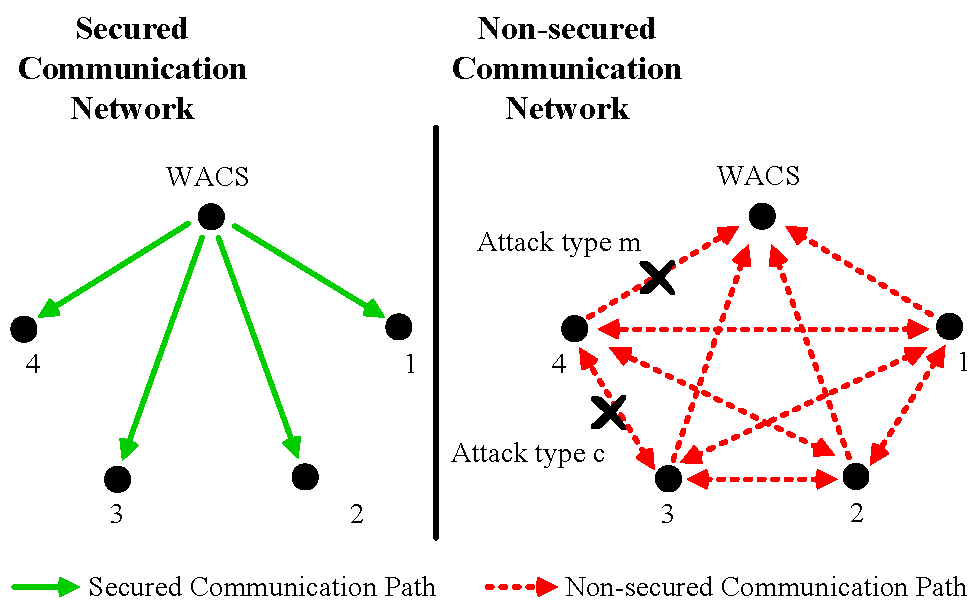
\includegraphics[scale=0.6]{chapters/se_nonlinear/figures/Comm_Net} \caption{A graphical depiction of the cyber network model: For simplicity, we focus on a system with only four generators in this figure. The graph in green (sold lines) shows the secured information flow (i.e., the set of information flows from the WACS to local controllers) while the graph in red (dotted lines) represents the set of non-secured information flows.}
\label{wacs}
\end{figure}

\subsection{Cyber Layer Model}
To maintain the system's stability, the system operator has equipped each generator with a local controller, PMU, and transceiver through which information can be exchanged with the local controllers of other generators as well as the WACS. These transceivers are connected through a communication network which sends PMU measurements, including rotors' speeds and generators' phase angles, to different transceivers. The communication network, PMUs, and transceivers are not secured, and hence they are subject to cyber attacks and communication failures.

In this study, we assume that the communication paths from the WACS to the local controllers are secured while other communication paths are not secured. Hence, the communication network interconnecting the transceivers can be described by two directed graphs, one for secured information flow and one for non-secured information flow, as shown in Figure~\ref{wacs}.


Typically, the WACS is strongly protected against cyber attacks, and the local transceivers are more vulnerable to cyber attacks and communication failures than the WACS. For more information, we refer the reader to the North American Electric Reliability Corp. (NERC)s Critical Infrastructure Protection (CIP) standards \cite{nerc}. In particular, we refer the reader to 1) CIP-002 BES Cyber System Categorization that identifies control centers as a ``High Impact Rating", and 2) CIP-005 Electronic security Perimeter(s) and CIP-006 Physical Security of BES Cyber Systems to see what requirements are needed for high impact systems. The CIP Standards explain why we assume that the communication paths from the WACS to the local controllers is secured.

%As mentioned earlier, in real power systems, measurements are telemetered from generating units to a wide area control system that performs secure state estimation and adjusts the set-point of each generator.
\textcolor{black}{To maintain the system's stability in the presence of attacks and failures, the WACS needs to perform secure state estimation before using the received data (e.g., $\omega_i$'s and $\theta_i$'s) for computing wide area control signals and for monitoring local controllers. To do so, we distinguish two types of attacks:
\begin{itemize}
\item \textbf{c-attack:} an attack that corrupts communication channels between local controllers.
\item \textbf{m-attack:} an attack that affects communication channels between a local controller and the WACS. %\textcolor{magenta}{ Is there any explanation/application such that we can justify $m$-attack? For example, any reviewers wonder why WACS $\rightarrow$ local controller is secured but local controller $\rightarrow$ WACS is non-secured.}
\end{itemize}
We assume that at any time instant, the cyber layer is subject to either a c-attack or an m-attack, but not both. This is discussed in detail in Section \ref{V_B}. However, both of these types of attacks and the set of attacked measurements can change at each time instant. These types of attacks are illustrated in Figure~\ref{wacs} for a power system comprising four generators.}



\textcolor{black}{Next, by using the proposed secure state estimation technique, we develop a secure state estimator for estimating the dynamic states (i.e., generator' phase angles and rotors' speeds) of the power network.}

%%%%%%%%%%%%%%%%%%%%%%%%%%%%%%%%%%%%%%%%%%%%%%%%%%%%%%%%%
%%%%%%%%%%%%%%%%%%%%%%%%%%%%%%%%%%%%%%%%%%%%%%%%%%%%%%%%%
%%%%%%%%%%%%%%%%%%%%%%%%%%%%%%%%%%%%%%%%%%%%%%%%%%%%%%%%%

\section{Secure State Estimator for Wide Area Control Systems}\label{sec:application1}
The system dynamics and power flows can be described by the algebraic differential equations in (\ref{load_bus})-(\ref{swing2k}). However, in order to use the proposed secure state estimation technique, we need to describe the system by a set of purely differential equations. To do so, we reduce the power network into a network of electro-mechanical oscillators, comprising the $G$ generators, by using the Kron reduction technique\footnote{\textcolor{black}{Kron reduction is a graph-based technique  used in power systems to eliminate algebraic load equations and to reduce the order of the interconnections between the synchronous generators \cite{kron}. This technique transforms an interconnected power system into an equivalent grid between the synchronous generators of the power system.}}. Let $\mathcal{V}^\prime$ denote the set of transmission lines between the $G$ generators after performing the Kron reduction technique, and let $\mathcal{K}(\mathcal{G},\mathcal{V}^\prime)$ denote the corresponding graph. This graph is connected and has $|\mathcal{V}^\prime|$ edges where $|\mathcal{V}^\prime| \le G (G-1)/2$.






We can now describe the power system by
\begin{equation}\label{eq:kron}
\begin{aligned}
\dot{\theta_i} & =\omega_i-\omega_0\\
\frac{2H_i}{\omega_0} \dot{\omega_i} &=P_i^m-\sum_{j\in\mathcal{N}_i}{{E_i E_j {|\widehat{y}_{ij}|} ~ \text{sin}(\theta_i-\theta_j+\widehat{\phi}_{ij})}}\\
&\quad-\textcolor{black}{\frac{d_i}{\omega_0} (\omega_i-\omega_0)}+ U_i
\end{aligned}
\end{equation}
where $\widehat{y}_{ij}=\widehat{g}_{ij}+\sqrt{-1} ~\widehat{b}_{ij}$ denotes the admittance of the Kron-reduced equivalent line between generators $i$ and $j$, and $\widehat{\phi}_{ij}$ equals $\text{arctan}(\widehat{g}_{ij}/\widehat{b}_{ij})$. $\mathcal{N}_i$ denotes the set of neighbors of generator $i$ in graph $\mathcal{K}(\mathcal{G},\mathcal{V}^\prime)$ (i.e., the reduced network).

In this study, we assume that the WACS performs a monitoring role and does secure estimation, and consider the mechanical input power $P_i^m$ and the storage control signal $U_i$ as local control signals which are computed based on PMU measurements and wide area control signals (e.g., area control error) \cite{Kundur}. When measurements are attacked, the estimated values of power flows or phase angles will not be equal to the actual values in the system (e.g., $P_{i,\text{meas}}^e \neq P_{i}^e$), and hence local controllers might send inaccurate signals to physical components. The WACS estimates attacks from measurements and communicates estimated attack signals to each generator. Then, each generator subtracts the estimated attack from the received measurements, as to obtain the most accurate values of $\omega_{i}$'s and $\theta_{i}$'s, and to make sure that the local controller will send accurate signals to the physical components that are under its control.




%%%%%%%%%%%%%%%%%%%%%%%%%%%%%%%%%
\vspace{-0.2cm}
\subsection{Formulation of Secure Estimation}

The local controller at generator $i$ computes the control input $U_i$ using (\ref{Eq:Ui}), in which $P_{i,\text{meas}}^e$ is calculated from PMU measurements:
\begin{equation}\label{eq:Pe_meas}
P_{i,\text{meas}}^e(t) = \sum_{j\in\mathcal{N}_i}{E_i E_j {|\widehat{y}_{ij}|} ~ \text{sin}\big(y^c_{ii}(t)-y^c_{ij}(t)+\widehat{\phi}_{ij}\big)},
\end{equation}
%In order to compute $P_{i,\text{meas}}^e$ and the local control signal $U_i$,
where $y^c_{ij}$ is the measured rotor angle of generator $j$ (i.e., $\theta_j$) received at generator $i$'s local controller. We assume that these PMU measurements are subject to attack:
\begin{equation}\label{Eq:yc}
\begin{aligned}
y^c_{ij}(t) & = \theta_j(t) + e^c_{ij} (t),~ i \in \mathcal{G},~j \in \mathcal{N}_i \cup \{i\}, \,
\end{aligned}
\end{equation}
where $e^c_{ij}$ represents the attack signal. As mentioned earlier, we refer to this as a c-attack (see Figure~\ref{wacs}).
%Note that $e^c_{ji}$ represents the corruption in the measurement of $\theta_i$ received at generator $j$, thus $e^c_{ij}$ and $e^c_{ji}$ represent two distinct variables.
In addition, we assume $e^c_{ii}(t) = 0$ for all $t$. Note that $\theta_i$ is measured locally, and therefore it is not subject to cyber attack, i.e., $y^c_{ii}(t) = \theta_i(t)$ for all $t$.
%Finally, $P^m_i$ represents the input mechanical power to generator $i$, thus is known to generator $i$.

%To enable the WACS to perform secure estimation, each generator sends all of its measurements to the WACS. In other words, the WACS receives the following measurements
To performs secure estimation, the WACS receives measurements $y^m_{ij}$ from all the local controllers. Since we assume the communication flows from the local controllers to the WACS are not secured, measurements $y^m_{ij}$ can be subject to attack:
\begin{equation}\label{Eq:ym}
\begin{aligned}
y^m_{ij}(t) &= y^c_{ij}(t) + e^m_{ij}(t),~i \in \mathcal{G},~j \in \mathcal{N}_i \cup \{i\} \,
\end{aligned}
\end{equation}
where $e^m_{ij}$ represents the corruption in $y^c_{ij}$. We refer to these attacks as m-attacks (see Figure~\ref{wacs}).

We now apply the forward Euler discretization scheme to this continuous-time system and obtain the following discrete-time approximation, assuming a constant discretization step $T_s$ for all $k$:
\begin{equation}
\begin{aligned}
\theta_i (k+1) &= \theta_i(k) + T_s \big(w_i(k) - \omega_0\big) \\
\omega_i(k+1)
	&= \alpha~\omega_i(k) + \beta \\
	& \quad + \sum_{j\in \mathcal{N}_i} f_{ij} \big(\theta_i(k), \theta_j(k), y^c_{ii}(k), y^c_{ij}(k)\big) \\
\end{aligned}
\end{equation}
where \textcolor{black}{$\alpha = 1- \frac{T_s (d_i + F_i)}{2H_i}$, $\beta = \frac{T_s  \omega_0(d_i+F_i)}{2H_i}$}, $f_{ij} (\cdot) = \tilde G_{ij} \big[ \sin \big(\theta_i(k) - \theta_j(k) + \widehat{\phi}_{ij}\big) - \sin \big(y^c_{ii}(k) - y^c_{ij}(k)+\widehat{\phi}_{ij}\big) \big] $
and $\tilde G_{ij} = - \frac{T_s \omega_0 E_i E_j |\widehat{y}_{ij}|}{2H_i}$.

Using (\ref{Eq:yc}) and (\ref{Eq:ym}), $f_{ij} (\cdot)$ can be re-written in terms of $y^m_{ij}$'s, which are the measurements received at the WACS, as follows:
\begin{equation} \label{Eq:case2_f_ij}
\begin{aligned}
	f_{ij} (\cdot ) &= \tilde G_{ij} \big[ \sin \big(\widehat{\phi}_{ij} + \theta_i(k) - \theta_j(k)\big) \\
		& \quad- \sin \big(\widehat{\phi}_{ij} + y^c_{ii}(k) - y^c_{ij}(k)\big) \big]\\
		& = \tilde G_{ij}  \sin \big(\widehat{\phi}_{ij} + y^m_{ii}(k) - y^m_{ij}(k) - e^m_{ii}(k) \\
		& \quad + e^m_{ij}(k) + e^c_{ij}(k)\big) - \tilde G_{ij} \sin \big(\widehat{\phi}_{ij} + y^m_{ii}(k) \\
		& \quad - y^m_{ij}(k) - e^m_{ii}(k) + e^m_{ij}(k)\big) \\
		& = G_{ij}^s (k) \epsilon_{ij}^c  (k)  -  G_{ij}^c  (k)  \epsilon_{ij}^s (k),
\end{aligned}\nonumber
\end{equation}
where $ G_{ij}^s(k) = \tilde G_{ij} \sin \big(\widehat{\phi}_{ij} + y^m_{ii}(k) - y^m_{ij}(k)\big)$, $ G_{ij}^c (k) = \tilde G_{ij} \cos \big(\widehat{\phi}_{ij} + y^m_{ii}(k) -y^m_{ij}(k)\big)$ are known to the WACS. On the other hand, $\epsilon_{ij}^c$ and $\epsilon_{ij}^s$ are functions of unknown attack signals and are defined as:
\begin{equation}\label{eq:epsilon_cs}
\begin{aligned}
\epsilon_{ij}^c(k) &= \cos \big(e^m_{ii}(k) - e^m_{ij}(k) - e^c_{ij}(k)\big) \\
& \quad - \cos \big(e^m_{ii}(k) - e^m_{ij}(k)\big) \\
\epsilon_{ij}^s (k) &= \sin \big(e^m_{ii}(k) - e^m_{ij}(k) - e^c_{ij}(k)\big) \\
& \quad - \sin \big(e^m_{ii}(k) - e^m_{ij}(k)\big).
\end{aligned}
\end{equation}
%In (\ref{Eq:case2_f_ij}), the second equality uses $\theta_{i}(k) = y^c_{ii}(k) = y^m_{ii}(k) - e^m_{ii}(k)$, $\theta_{j}(k) = y^c_{ij}(k) - e^c_{ij}(k) = y^m_{ij}(k) - e^m_{ij}(k) - e^c_{ij}(k)$.
In other words, $f_{ij}(\cdot)$ is now a linear function of the unknowns: $\epsilon_{ij}^c(k)$ and $\epsilon_{ij}^s(k)$, whose coefficients can be computed by the WACS from the received measurements. In addition, if there is no attack on any of the communication channels in the system at time slot $k$, then $\epsilon_{ij}^c (k) = \epsilon_{ij}^s (k) = 0$.

The state space model of the $i$-th generator is given by:
\begin{equation}
\begin{aligned}
x_i(k+1) &= A_i x_i(k) + q_i + H_i(k) \epsilon_i(k) \\
& = \begin{bmatrix} 1 & T_s \\ 0 & \alpha \end{bmatrix} x_i(k) + \begin{bmatrix} -T_s \omega_0 \\ \beta \end{bmatrix} + \begin{bmatrix} 0 \\ h_i(k)^\top \end{bmatrix} \epsilon_i(k)
%y_i(k) &= C_i x_i(k) \\
\end{aligned}
\end{equation}
where the state vector $ x_i(k) = \begin{bmatrix}  \theta_i(k), \omega_i(k) \end{bmatrix}^\top$ and
\begin{equation}
\begin{aligned}
h_i(k)^\top & = \big[ G_{i\mathcal{N}_i(1)}^s(k), \cdots, G_{i\mathcal{N}_i(l_i)}^s(k), \\
& \quad \quad \quad G_{i\mathcal{N}_i(1)}^c(k),  \cdots,  G_{i\mathcal{N}_i(l_i)}^c(k) \big] \in \mathbb{R}^{1 \times 2l_i}\\
\epsilon_i(k) & =  \big[\epsilon_{i\mathcal{N}_i(1)}^c(k), \cdots , \epsilon_{i\mathcal{N}_i(l_i)}^c(k), \\
& \quad\quad\quad \epsilon_{i\mathcal{N}_i(1)}^s (k), \cdots, \epsilon_{i\mathcal{N}_i(l_i)}^s (k) \big] ^\top \in \mathbb{R}^{2l_i \times 1}.
\end{aligned}\nonumber
\end{equation}
Here, $\mathcal{N}_i(j)$ is the $j$-th generator in the neighborhood of generator $i$ and $l_i$ is the cardinality of the set $\mathcal{N}_i$.
%$H_i(k) \triangleq \begin{bmatrix} 0_{1 \times 2l_i} \\ h_i(k)^\top \end{bmatrix} \in \mathbb{R}^{2 \times 2l_i}$, where $h_i(k)^\top = \begin{bmatrix} G_{i\mathcal{N}_i(1)}^s(k), \cdots, G_{i\mathcal{N}_i(l_i)}^s(k), G_{i\mathcal{N}_i(1)}^c(k),  \cdots,  G_{i\mathcal{N}_i(l_i)}^c(k) \end{bmatrix} \in \mathbb{R}^{1 \times 2l_i}$. Here $\mathcal{N}_i(j)$ presents the $j$-th node in the neighborhood of generator $i$ and $l_i$ represents the cardinality of the set $\mathcal{N}_i$.

Consider the enlarged system with $G$ generators in the network:
\begin{equation}\label{eq:state_space_N}
\begin{aligned}
X(k+1) & = AX(k) + q + H(k) \epsilon(k) \\
Y(k) & = CX(k) + DE(k)
\end{aligned}
\end{equation}
where
\begin{equation}
\begin{aligned}
X(k) &= \begin{bmatrix} x_1(k); \cdots; x_G(k) \end{bmatrix} \in \mathbb{R}^{2G\times 1} \\
A &= \text{blkdiag} \{ A_1, \cdots, A_G\} \in \mathbb{R}^{2G\times 2G}\\
q &= \begin{bmatrix} q_1; \cdots; q_G \end{bmatrix} \in \mathbb{R}^{2G\times 1}\\
H(k)& = \text{blkdiag} \{ H_1(k), \cdots, H_G(k) \}  \in \mathbb{R}^{2G\times 4L }\\
\epsilon(k) &\triangleq \begin{bmatrix} \epsilon_1(k); \cdots; \epsilon_G(k)\end{bmatrix} \in \mathbb{R}^{4L \times 1}  \\
Y(k) &= \begin{bmatrix} Y_{i}(k); \cdots; Y_G(k) \end{bmatrix} \in \mathbb{R}^{(G+2L) \times 1} \\
Y_i(k) & = \begin{bmatrix} y_{ii}(k); y_{i\mathcal{N}_i(1)}(k); \cdots; y_{i\mathcal{N}_i(l_i)}(k) \end{bmatrix} \in \mathbb{R}^{(1+l_i) \times 1} \\
%C &\triangleq \begin{bmatrix} C^1; \cdots; C^G\end{bmatrix}  \in \mathbb{R}^{(N+2L)\times 2N}\\
D &= \begin{bmatrix} D_1, D_2 \end{bmatrix}  \in \mathbb{R}^{(G+2L)\times (G+4L)}\\
%D_1 &\triangleq \text{blkdiag} \{d_1, \cdots, d_G\} \in \mathbb{R}^{(N+2L) \times 2L} \\
D_1 &= \text{blkdiag} \left \{ \begin{bmatrix} 0 \\ I_{l_1, l_1} \end{bmatrix}, \cdots, \begin{bmatrix} 0 \\ I_{l_G, l_G} \end{bmatrix} \right \} \in \mathbb{R}^{(G+2L) \times 2L} \\
D_2 & = I_{G+2L, G+2L} \in \mathbb{R}^{(G+2L) \times (G+2L)} \\
E(k) &=  \begin{bmatrix} E^c_1(k); \cdots; E^c_G(k); E^m_1(k) ; \cdots;  E^m_G(k) \end{bmatrix} \\
& \quad\in \mathbb{R}^{(G+4L) \times 1} \\
E^c_i(k) & = \begin{bmatrix} e^c_{i\mathcal{N}_i(1)}(k); \cdots; e^c_{i\mathcal{N}_i(l_i)}(k) \end{bmatrix} \in \mathbb{R}^{l_i \times 1} \\
E^m_i(k) & = \begin{bmatrix} e^m_{ii}; e^m_{i\mathcal{N}_i(1)}(k); \cdots; e^m_{i\mathcal{N}_i(l_i)}(k) \end{bmatrix} \in \mathbb{R}^{(1+l_i) \times 1}
\end{aligned}\nonumber
\end{equation}
and $L = \frac{\sum_i l_i}{2}$ represents the total number of edges / links in the network. Matrix $C \in \mathbb{R}^{(G+2L)\times 2G}$ is given as follows: let the $a$-th element of vector $Y$ be $y^m_{ij}$, then the $(a,b)$-th entry of $C$ is given by
\begin{equation}
C_{(a,b)} = \begin{cases}1 & \mbox{if } 2j-1 = b \\ 0 & \mbox{otherwise.} \end{cases} \nonumber
\end{equation}

\noindent
Consider $T$ time steps of measurements (i.e., $k = \{0, \cdots, T-1 \}$) and define:
\begin{equation}
\bar Y = \begin{bmatrix} Y (0)  \\ Y (1) - C q  \\ \vdots \\ Y(T-1) - C \sum_{m=0}^{T-2}A^{T-2-m} q \end{bmatrix} \in \mathbb{R}^{(G+2L)T \times 1}
\end{equation}
then
\begin{equation}\label{eq:Ebar_Psi}
\bar Y = \Phi X(0) + \Psi  \bar E
\end{equation}
where $\Phi = \begin{bmatrix} C; CA ; \cdots ; CA^{T-1} \end{bmatrix} \in \mathbb{R}^{(G+2L)T \times 2G}$ is \textcolor{black}{the $T$-step observability matrix of the system}, $\bar E = \begin{bmatrix} E(0); \cdots; E(T-1); \epsilon(0); \cdots; \epsilon(T-2) \end{bmatrix} \in \mathbb{R}^{((G+4L)T + 4L(T-1)) \times 1} $ and $\Psi = \begin{bmatrix} \Psi_{1} & \Psi_{2} \end{bmatrix}$, with $\Psi_{1} \in \mathbb{R}^{(G+2L)T \times (G+4L)T}$ and $\Psi_{2}\in \mathbb{R}^{(G+2L)T \times 4L(T-1)}$ as follows:
\begin{equation}
\begin{aligned}
\Psi_{1} &= \text{blkdiag} \{ D, \cdots, D \} \\
\Psi_{2} &= \begin{bmatrix}   0 &  0  &  \cdots    	\\
   			        C H(0) & 0 &  \cdots  	\\
			       CAH(0) &  CH(1) & \cdots	\\
			        \vdots & \vdots  &  \ddots \\
			       CA^{T-2}H(0) & \cdots & CH(T-2) \\			
			    \end{bmatrix}	.
\end{aligned}\nonumber
\end{equation}

\noindent
We can choose $\Omega \in \mathbb{R}^{ ((G+2L)T - 2G)\times (G+2L)T}$ such that $\Omega \Phi = 0$, then:
\begin{equation}\label{eq:Ebar_OmegaPsi}
	\tilde Y = \Omega \bar Y = \Omega \Psi \bar E,
\end{equation}
where $\Omega \Psi \in \mathbb{R}^{((G+2L)T - 2G) \times ((G+4L)T + 4L(T-1))}$.

%%%%%%%%%%%%%%%%%%%%%%%%%%%%%%

\subsection{Challenges in Secure Estimation due to the Power System's Dynamics}\label{V_B}
The linear system in (\ref{eq:Ebar_OmegaPsi}) is in the form of (\ref{eq:E_est}). Hence, from Lemma \ref{lem:CS}, $\bar E$ has a unique $s$-sparse solution if all subsets of $2s$ columns of  $\Omega\Psi$ are linearly independent.
We now explain that this is not the case in the power systems example as some columns of $\Psi$ are linearly dependent.
Let us begin with the following: consider a matrix-vector multiplication $M \cdot v$, where $M = [ m_1, \cdots, m_n ] \in \mathbb{R}^{l \times n}$ and $m_i$ is the $i$-th column of $M$, $v = [ v_1, \cdots, v_n ] ^\top \in \mathbb{R}^{n \times 1}$, and $v_i$ is the $i$-th entry of $v$. In the sequel, the phrase ``the column of $M$ that corresponds to $v_i$" refers to the column of $M$ that multiplies the $v_i$ entry in the matrix-vector multiplication, i.e., $m_i$.

We now explain why $\Psi_2$ is rank deficient.
Observe that for all $i$ and $k$, the first row of $H_i(k)$ is equal to zero. Therefore given any matrix $M = \begin{bmatrix} m_1 & m_2 \end{bmatrix} \in \mathbb{R}^{l \times 2}$, where $m_1$ and $m_2$ are the columns of $M$, we have:
\textcolor{black}{\begin{align}
\operatorname{rank} \big( M \cdot H_i(k) \big) &=  \operatorname{rank} \left( \begin{bmatrix} m_1 & m_2  \end{bmatrix} \cdot \begin{bmatrix} 0 & 0 & \cdots \\ h_{21} & h_{22} & \cdots \end{bmatrix} \right)\nonumber\\
	= &\operatorname{rank} \left( \begin{bmatrix} h_{21} m_2 & h_{22} m_2 & \cdots \end{bmatrix} \right)=1.
\end{align}}
Since $H(k)$ is block diagonal, we can show that $\Psi_2$ is also rank deficient.
%To see this more clearly, the first row of $H_i(k)$ are zeros, therefore given any matrix $M$, $\text{rank}(MH_i(k)) = 1$. In other words, all columns of $\Psi_2$ that correspond to the same $H_i(k)$ are linearly dependent. In (\ref{eq:Ebar_OmegaPsi}), $\Psi_2$ multiplies the $\epsilon(k)$ terms in $\bar E$, consequently, the $\epsilon(k)$'s may not be identifiable.
Next, from (\ref{Eq:yc}) and (\ref{Eq:ym}), we have $y^m_{ij}(k) = \theta_j(k) + e^c_{ij}(k) + e^m_{ij}(k)$, which means for a given ($i,j$)-pair ($i \neq j$) and a given time slot $k$, the two columns of $\Psi_1$ that correspond to the two terms $e^c_{ij}(k)$ and $e^m_{ij}(k)$ in $\bar E$ are identical, i.e., linearly dependent. Therefore, by Lemma \ref{lem:CS}, the solution $\bar E$ obtained by solving (\ref{eq:Ebar_OmegaPsi}) (i.e., the estimation algorithm introduced in Section \ref{sec:SE}) is not unique.
Does this mean we can not uniquely recover the attack signal?
A closer analysis reveals the specific entries in $\bar E$ that cannot be uniquely identified, and shines light on how to overcome this challenge. Our observations are as follows:
\begin{enumerate}
\item Observe from (\ref{eq:Ebar_OmegaPsi}) that $\Psi_2$ multiplies the $\epsilon(k)$ terms in $\bar E$, i.e., $\big( \epsilon(0), \cdots, \epsilon(T-2) \big)$.
Linear dependence of the columns of $\Psi_2$ causes the $\epsilon(k)$ terms to be unidentifiable.
However, $\epsilon (k)$ can be computed from $E(k)$ using (\ref{eq:epsilon_cs}). In other words, although the $\epsilon(k)$ terms in the solution $\bar E$ are not unique, as long as the $E(k)$ terms in $\bar E$ are unique, then we can determine the $\epsilon (k)$ terms uniquely using (\ref{eq:epsilon_cs}).

\item The identical columns of $\Psi_1$ that correspond to the two terms $e^c_{ij}(k)$ and $e^m_{ij}(k)$ in $\bar E$ means that it is only possible to uniquely identify the sum $e^c_{ij}(k)+e^m_{ij}(k)$, but not the individual terms: $e^c_{ij}(k)$ and $e^m_{ij}(k)$. To overcome this challenge, we make the assumption that at any time $k$, the system is subject to either a c-attack or an m-attack, but not both. In other words, $e^m_{ij}(k)$ and $e^c_{ij}(k)$ cannot both be non-zero, thus making them identifiable.
\end{enumerate}
Next, we explain our secure estimation algorithm.

%%%%%%%%%%%%%%%%%%%%%%%%%%%%%%%

\subsection{Assumptions and Secure Estimation with 2-Step Delay}


As mentioned earlier, we assume that at any time slot $k$, the cyber layer is subject to either a c-attack or an m-attack, but not both at the same time.
However, both the types of attacks and the set of attacked measurements can change at each time step. In addition, the WACS does not know \textit{a priori} which type of attack the network is subjected to. Hence, secure estimation techniques are required to determine the type of attack, as well as the exact corruption signals.

Using the difference equation in (\ref{eq:state_space_N}), we find that
\textcolor{black}{
\begin{align}\label{eq:2step_delay}
&f_\text{2-step}\big (\epsilon(k-2), E(k) \big)  = Y(k) - CA^2\cdot X(k-2) - CAq  \nonumber\\
	&   - Cq - CA\cdot H(k-2)\cdot \epsilon(k-2)  - DE(k)= 0
\end{align}}
where the first equality uses $CH(k)=0$ for all $k$. Observe that if it is an m-attack at time $k$, then $e^c_{ij}(k) = 0$ and $e^c_{ij}(k) + e^m_{ij}(k) = e^m_{ij}(k)$, furthermore, $\epsilon(k) = 0$. On the other hand, if it is a c-attack at time $k$, then $e^m_{ij}(k) = 0$ and $e^c_{ij}(k) + e^m_{ij}(k) = e^c_{ij}(k)$, in addition, $\epsilon(k) \neq 0$.
Combining these two observations with (\ref{eq:2step_delay}), we propose the following algorithm which can be used by the WACS to determine the type of attack and the exact corruption signals, with a 2-step delay.

We first introduce some notation used in the algorithm. Let $E_\text{b}(k)$ denote the estimated vector $E(k)$ without imposing the assumption that only a c-attack or an m-attack can occur.  $E_{\text{c-att}}(k)$ and $E_{\text{m-att}}(k)$ denote the estimated vector $E(k)$ if it is a c-attack or an m-attack at time $k$, respectively, and can be computed from $E_\text{b}(k)$. For example, to obtain $E_{\text{c-att}}(k)$, we set all $e^m_{ij}$ terms in $E_{\text{c-att}}(k)$ to zero, and set all $e^c_{ij}$ terms equal to the sum of corresponding $e^c_{ij}$ and $e^m_{ij}$ terms in $E_\text{b}(k)$. We can obtain $E_{\text{m-att}}(k)$ in a similar fashion. Finally, $\epsilon_{\text{c-att}}(k)$ and $\epsilon_{\text{m-att}}(k)$ are the $\epsilon(k)$ vectors computed from $E_{\text{c-att}}(k)$ and $E_{\text{m-att}}(k)$, respectively.
With these notations in hand, we now present our estimation algorithm in Algorithm \ref{al:se}.


\begin{algorithm}
\caption{Secure Estimation}
\label{al:se}
\begin{algorithmic}[1]
%\State Initialize the KF
\For{each $k$}
	\State Estimate $\bar E(k)$ by solving the following $l_1$-minimization problem:
		\begin{equation}
		\bar E_\text{b}(k) = \arg \min \| \bar E \|_{l_1} ~\text{subject to}~ \tilde Y = \Omega\Psi \bar E.
		\nonumber
		\end{equation}
	\State Extract $E_\text{b}(k-2)$ and $E_\text{b}(k)$ from $\bar E_\text{b}(k)$.
	\State Evaluate equation (\ref{eq:2step_delay}) for the case with an m-attack at time $k-2$, using the observation that $\epsilon_\text{m-att}(k-2) = 0$.
	\State Evaluate equation (\ref{eq:2step_delay}) for the case with a c-attack at time $k-2$, by first computing $E_\text{c-att}(k-2)$ and then use (\ref{eq:epsilon_cs}) to obtain $\epsilon_\text{c-att}(k-2)$.
	\If{$\|f_\text{2-step}\big (\epsilon_\text{c-att}(k-2), E_\text{b}(k) \big) \| < \|f_\text{2-step}\big (\epsilon_\text{m-att}(k-2), E_\text{b}(k) \big) \|$}
		\State It is a c-attack at $k-2$: $E(k-2) = E_\text{c-att}(k-2)$ and $\epsilon(k-2) = \epsilon_\text{c-att}(k-2)$
	\Else
		\State It is an m-attack at $k-2$: $E(k-2) = E_\text{m-att}(k-2)$ and $\epsilon(k-2) = \epsilon_\text{m-att}(k-2)= 0$
	\EndIf
\EndFor
\end{algorithmic}
\end{algorithm}



To summarize, as a result of the system dynamics and the proposed model, it is not possible to recover the exact corruption if the system is subjected to both c- and m-attacks at the same time. In light of this, we make the simplifying assumption that at any time $k$, the system may only be subject to one type of attack. However, the type of attack can change over time. Then, by comparing the actual measurements with the system trajectories that would result from each type of attack, we can determine both the attack type and the exact corruption signals, with a 2-step delay. Note that at time $k$, this secure state estimation algorithm is able to detect the presence of attacks at times $k-1$ and $k$, merely not the exact attack signals.
Next, we numerically demonstrate the effectiveness of the proposed state estimation algorithm.




